% ============================================================
% Cheat sheet, argomento 6: dal codice al diagramma, ereditarietà, interfacce e tipi speciali
% ============================================================
\argomento{Dal codice al diagramma: ereditarietà, interfacce, tipi speciali}{Dispensa: capitolo 7. extends,
implements, enum, e i costrutti che le slide non mostrano}[Dal codice: ereditarietà e tipi speciali]

\begin{caso}{ereditarieta}{extends: la generalizzazione}
\begin{lstlisting}[style=javacs]
class Veicolo {
    protected String targa;
    public void avvia() { }
}
class Auto extends Veicolo {
    private int porte;
    @Override
    public void avvia() { }   // ridefinito
}
class Moto extends Veicolo {
    private boolean bauletto;
}
\end{lstlisting}
\tcblower
\begin{tikzpicture}
  \umlclass[2.6cm]{v}{(0,0)}{Veicolo}{\# targa: String}{+ avvia()}
  \umlclass[2.4cm]{a}{(-1.6,-2.4)}{Auto}{- porte: int}{+ avvia()}
  \umlclass[2.6cm]{m}{(1.6,-2.4)}{Moto}{- bauletto: boolean}{}
  \coordinate (t) at (0,-1.3);
  \draw[gen] (t) -- (v.south);
  \draw[assocl] (a.north) |- (t) -| (m.north);
\end{tikzpicture}
\regola{Una freccia a triangolo vuoto da ogni sottoclasse alla superclasse (le punte si possono unire in una
sola). La sottoclasse mostra solo ciò che \textbf{aggiunge} (\code{porte}) e ciò che \textbf{ridefinisce}
(\code{avvia}); \code{targa} è ereditato e non si ripete. \code{protected} $\to$ \code{\#}.}
\end{caso}

\begin{caso}{realizzazionecodice}{implements: la realizzazione, anche di più interfacce}
\begin{lstlisting}[style=javacs]
interface Stampabile {
    void stampa();
}
interface Salvabile {
    void salva(String file);
}
class Documento implements Stampabile, Salvabile {
    public void stampa() { }
    public void salva(String file) { }
}
\end{lstlisting}
\tcblower
\begin{tikzpicture}
  \umlclass[2.4cm]{s1}{(-1.5,0)}{\stereotipo{interface}{Stampabile}}{}{+ stampa()}
  \umlclass[2.6cm]{s2}{(1.6,0)}{\stereotipo{interface}{Salvabile}}{}{+ salva(file: String)}
  \umlclass[2.6cm]{d}{(0,-2.5)}{Documento}{}{+ stampa()\\+ salva(file: String)}
  \draw[realizza] ($(d.north)+(-0.5,0)$) -- ++(0,0.4) -| (s1.south);
  \draw[realizza] ($(d.north)+(0.5,0)$) -- ++(0,0.4) -| (s2.south);
  % la stessa cosa con le palline
  \node[classe1=1.9cm] (d2) at (4.4,-2.5) {Documento};
  \draw[assocl] ($(d2.north)+(-0.4,0)$) -- ++(0,0.5);
  \palla{($(d2.north)+(-0.4,0.61)$)}
  \node[ruolo, anchor=south] at ($(d2.north)+(-0.4,0.72)$) {Stampabile};
  \draw[assocl] ($(d2.north)+(0.4,0)$) -- ++(0,1.1);
  \palla{($(d2.north)+(0.4,1.21)$)}
  \node[ruolo, anchor=south] at ($(d2.north)+(0.4,1.32)$) {Salvabile};
\end{tikzpicture}
\regola{Freccia \textbf{tratteggiata} con il triangolo vuoto verso ogni interfaccia implementata; la classe elenca i
metodi che implementa. A destra la forma abbreviata a palline (\vv{lollipop}): stesso significato.}
\end{caso}

\begin{caso}{estendeimplementa}{extends e implements insieme}
\begin{lstlisting}[style=javacs]
abstract class Persona {
    protected String nome;
}
interface Cassiere {
    void incassa(double euro);
}
class Impiegato extends Persona
                implements Cassiere {
    public void incassa(double euro) { }
}
\end{lstlisting}
\tcblower
\begin{tikzpicture}
  \umlclass[2.4cm]{p}{(-1.6,0)}{\textit{Persona}}{\# nome: String}{}
  \umlclass[3.2cm]{c}{(1.9,0)}{\stereotipo{interface}{Cassiere}}{}{+ incassa(euro: double)}
  \umlclass[3.2cm]{i}{(0,-2.6)}{Impiegato}{}{+ incassa(euro: double)}
  \draw[gen] ($(i.north)+(-0.5,0)$) |- ++(0,0.45) -| (p.south);
  \draw[realizza] ($(i.north)+(0.5,0)$) |- ++(0,0.45) -| (c.south);
\end{tikzpicture}
\regola{Una sola superclasse (linea continua) e quante interfacce si vuole (tratteggiate): in Java si eredita da
\textbf{una} classe sola. Classe astratta in corsivo.}
\end{caso}

\begin{caso}{interfacciaestende}{Un'interfaccia che ne estende un'altra}
\begin{lstlisting}[style=javacs]
interface Forma {
    double area();
}
interface Forma3D extends Forma {
    double volume();
}
class Cubo implements Forma3D {
    private double lato;
    public double area() { return 6 * lato * lato; }
    public double volume() {
        return lato * lato * lato;
    }
}
\end{lstlisting}
\tcblower
\begin{tikzpicture}
  \umlclass[2.6cm]{f}{(0,0)}{\stereotipo{interface}{Forma}}{}{+ area(): double}
  \umlclass[2.6cm]{f3}{(0,-2.2)}{\stereotipo{interface}{Forma3D}}{}{+ volume(): double}
  \umlclass[2.6cm]{c}{(3.6,-2.2)}{Cubo}{- lato: double}{+ area(): double\\+ volume(): double}
  \draw[gen] (f3.north) -- (f.south);
  \draw[realizza] (c.west) -- (f3.east);
\end{tikzpicture}
\regola{Fra due interfacce \code{extends} è una \textbf{generalizzazione}: linea \textbf{continua}. Fra classe e
interfaccia \code{implements} è una \textbf{realizzazione}: linea \textbf{tratteggiata}. Il \code{Cubo} deve
implementare i metodi di entrambe.}
\end{caso}

\begin{caso}{enumcampi}{Enumerazioni con campi e metodi \oltre}
\begin{lstlisting}[style=javacs]
enum Taglia {
    S(44), M(48), L(52);

    private final int numero;
    Taglia(int numero) { this.numero = numero; }
    int getNumero() { return numero; }
}
\end{lstlisting}
\tcblower
\begin{tikzpicture}
  \node[rectangle split, rectangle split parts=4, draw=q9!75!black, fill=yellow!10, line width=0.7pt,
        font=\scriptsize, text width=3.2cm, align=left, inner sep=2.5pt] (t) at (0,0)
        {\centering{\tiny«enumeration»}\\\textbf{Taglia}\par\nodepart{two}S\\M\\L
         \nodepart{three}- numero: int \{readOnly\}\nodepart{four}\textasciitilde\ getNumero(): int};
  \node[ruolo, anchor=west, text=swgray] at ($(t.two east)+(0.1,0)$) {letterali};
  \node[ruolo, anchor=west, text=swgray] at ($(t.three east)+(0.1,0)$) {attributi};
  \node[ruolo, anchor=west, text=swgray] at ($(t.four east)+(0.1,0)$) {operazioni};
\end{tikzpicture}
\regola{Un'\code{enum} di Java può avere campi, costruttore e metodi: l'enumerazione UML ha allora uno scomparto per i
\textbf{letterali} e, sotto, quelli soliti per attributi e operazioni. Il costruttore (sempre privato) di solito non
si disegna.}
\end{caso}

\begin{caso}{generica}{Classi generiche \oltre}
\begin{lstlisting}[style=javacs]
class Scatola<T> {
    private T contenuto;
    void metti(T x) { contenuto = x; }
    T prendi() { return contenuto; }
}
class Libro { }
class Biblioteca {
    private final Scatola<Libro> deposito =
            new Scatola<>();
}
\end{lstlisting}
\tcblower
\begin{tikzpicture}
  \umlclass[2.6cm]{s}{(0,0)}{Scatola}{- contenuto: T}{\textasciitilde\ metti(x: T)\\\textasciitilde\ prendi(): T}
  \node[draw=black!80, dashed, fill=white, font=\tiny, inner sep=2pt] at ($(s.north east)+(-0.1,0.02)$) {T};
  \umlclass[3.8cm]{b}{(4.4,0)}{Biblioteca}{- deposito: Scatola<Libro>}{}
\end{tikzpicture}
\regola{Il parametro di tipo \code{T} va nel rettangolo \textbf{tratteggiato} in alto a destra; dentro la classe
\code{T} si usa come un tipo qualunque. Dove la classe si usa con un tipo concreto basta scrivere
\code{Scatola<Libro>} come tipo dell'attributo (oppure \code{«bind»}, \vv{template}).}
\end{caso}

\begin{caso}{annidatacodice}{Classi annidate e interne \oltre}
\begin{lstlisting}[style=javacs]
class Ordine {
    private final List<Riga> righe =
            new ArrayList<>();

    class Riga {               // classe interna
        private String prodotto;
        private int quantita;
    }
    void aggiungi(String p, int q) {
        Riga r = new Riga();
        r.prodotto = p;
        r.quantita = q;
        righe.add(r);
    }
}
\end{lstlisting}
\tcblower
\begin{tikzpicture}
  \umlclass[3.8cm]{o}{(0,0)}{Ordine}{}{\textasciitilde\ aggiungi(p: String, q: int)}
  \umlclass[2.6cm]{r}{(5.2,0)}{Ordine::Riga}{- prodotto: String\\- quantita: int}{}
  \draw[compos] ($(o.east)+(0,0.25)$) -- ($(r.west)+(0,0.25)$);
  \node[molt, anchor=south east] at ($(r.west)+(-0.1,0.32)$) {* \{ordered\}};
  \node[ruolo, anchor=north east] at ($(r.west)+(-0.1,0.18)$) {righe};
  \draw[annida] ($(o.east)+(0,-0.3)$) -- ($(r.west)+(0,-0.3)$);
  \piuAnnida{($(o.east)+(0.13,-0.3)$)}
\end{tikzpicture}
\regola{Che \code{Riga} sia dichiarata \textbf{dentro} \code{Ordine} si mostra con il cerchio con la croce (oppure con
il nome \code{Ordine::Riga}). È un'informazione sul codice, non sui legami fra oggetti: la lista \code{righe} va
disegnata a parte, qui come \textbf{composizione} (le righe nascono dentro l'ordine e non escono).}
\end{caso}

\begin{caso}{record}{Record \oltre}
\begin{lstlisting}[style=javacs]
record Punto(int x, int y) {
    double distanza() {
        return Math.sqrt(x * x + y * y);
    }
}
\end{lstlisting}
\tcblower
\begin{tikzpicture}
  \umlclass[3.2cm]{p}{(0,0)}{\stereotipo{record}{Punto}}{- x: int \{readOnly\}\\- y: int \{readOnly\}}{\textasciitilde\ Punto(x: int, y: int)\\+ x(): int\\+ y(): int\\\textasciitilde\ distanza(): double}
\end{tikzpicture}
\regola{Un \code{record} è una classe \code{final} con un campo \code{private final} per ogni componente, un
costruttore con tutti i componenti (con la visibilità del record: qui di package) e un metodo di accesso
\code{public} per ciascuno (\code{x()}, \code{y()}): attributi \code{\{readOnly\}}. Lo stereotipo «record» non è
standard ma si capisce; metodi d'accesso e costruttore si possono omettere.}
\end{caso}

\begin{caso}{default}{Interfacce con metodi default e statici \oltre}
\begin{lstlisting}[style=javacs]
interface Saluto {
    String nome();                     // astratto
    default String saluta() {          // con corpo
        return "Ciao " + nome();
    }
    static Saluto di(String n) {       // statico
        return () -> n;
    }
}
\end{lstlisting}
\tcblower
\begin{tikzpicture}
  \umlclass[3.8cm]{s}{(0,0)}{\stereotipo{interface}{Saluto}}{}{+ \textit{nome(): String}\\+ saluta(): String\\\underline{+ di(n: String): Saluto}}
\end{tikzpicture}
\regola{In un'interfaccia le operazioni sono astratte e di solito non si scrivono in corsivo; se ci sono metodi
\code{default}, il corsivo distingue quelli \textbf{senza} corpo. Il metodo \code{static} si sottolinea. Nelle
interfacce tutto è \code{public}.}
\end{caso}

\begin{caso}{eccezione}{Eccezioni personalizzate \oltre}
\begin{lstlisting}[style=javacs]
class SaldoInsufficiente extends Exception {
    SaldoInsufficiente(String msg) { super(msg); }
}
class Conto {
    private double saldo;
    void preleva(double x)
            throws SaldoInsufficiente {
        if (x > saldo)
            throw new SaldoInsufficiente("poco");
        saldo -= x;
    }
}
\end{lstlisting}
\tcblower
\begin{tikzpicture}
  \node[classe1=2.0cm] (e) at (0,0) {Exception};
  \node[classe1=2.6cm] (s) at (0,-1.6) {SaldoInsufficiente};
  \umlclass[3.0cm]{c}{(4.6,-1.6)}{Conto}{- saldo: double}{\textasciitilde\ preleva(x: double)}
  \draw[gen] (s.north) -- (e.south);
  \draw[dep] (c.west) -- node[stereo, above]{«create»} (s.east);
\end{tikzpicture}
\regola{Un'eccezione è una classe come le altre: \code{extends Exception} è una generalizzazione verso la classe di
libreria (si disegna solo il nome). \code{Conto} la crea con \code{throw new}: dipendenza «create». La clausola
\code{throws} non ha un simbolo nelle slide; se serve, si scrive in una nota.}
\end{caso}
